\section{Methodology}
\label{sec:method}
%\FloatBarrier

As described in Section~\ref{sec:problem}, the input data comes in the form of a
PDF file which can be converted into plaintext XML data containing lines of text
along with each line's bounding box. There are two systems in play here; the
main system is a convolutional neural network classifier that acts on the XML
data. Further details on this are provided in Section~\ref{sec:sup}. The second
system is the unsupervised preprocessor whichs acts on the PDF data and writes
its output as an additional property into the XML data, which is elaborated upon
in Section~\ref{sec:unsup}. Figure~\ref{fig:overview} shows a high-level
overview of the two systems and how they interact.

\begin{figure}[htb]
  \centering
  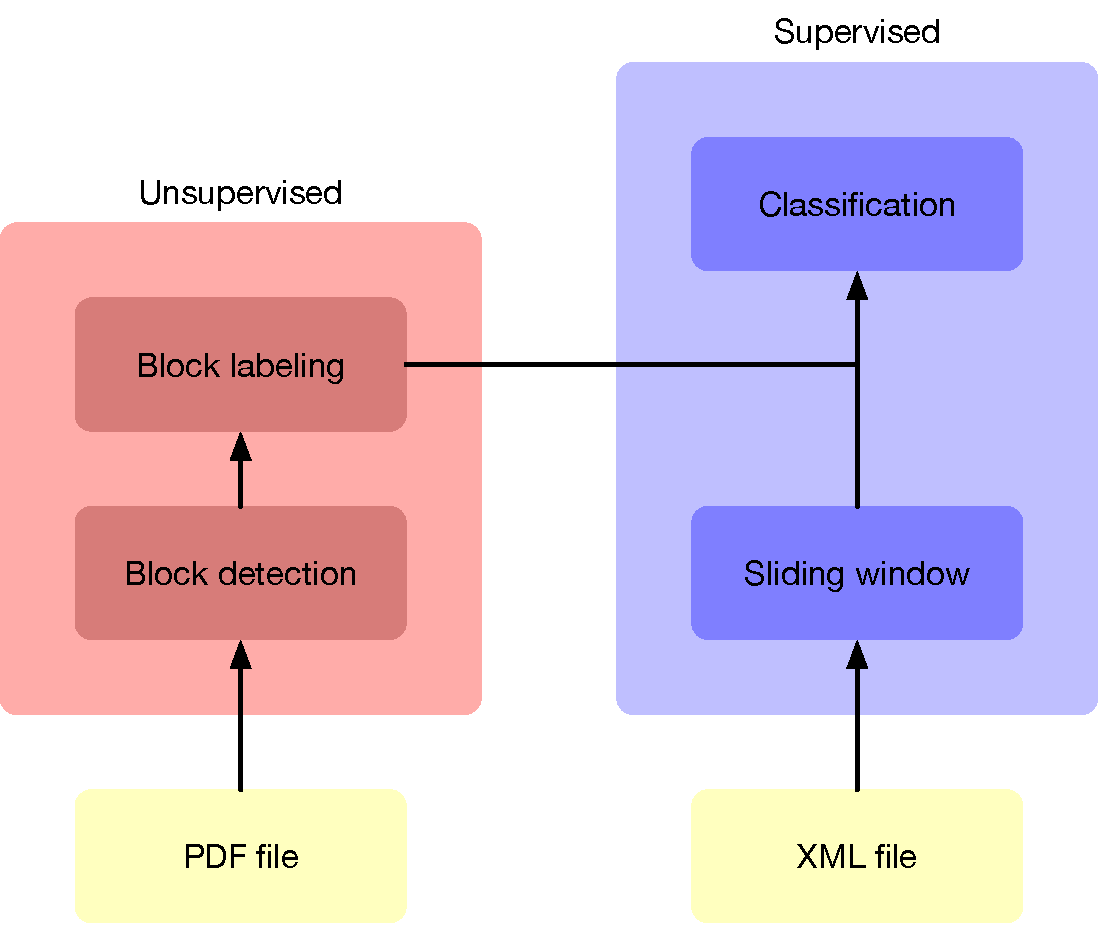
\includegraphics[width=\textwidth]{figures/layout.pdf}
  \caption{A high-level overview of the system. The unsupervised block augments
  the input to the classifier.}
  \label{fig:overview}
\end{figure}

\subsection{Unsupervised}
\label{sec:unsup}
The unsupervised algorithm intends to detect and classify blocks of text in the
PDF file; Figure~\ref{fig:clustered} shows an example. This approach is based on
work by \textcite{klampfl2014unsupervised}, and consists of two separate
clustering steps. First, individual characters (the fundamental objects
available in a PDF file) are clustered together into blocks of semantically
relevant text. These would be paragraphs, section headers, page decoration, etc.
By using the bounding boxes of the blocks, they can be clustered based on their
shape and some additional metadata (e.g.\ occurrence of font types and sizes).
The next two subsections will go into details on the two clustering steps.

\begin{figure}[htb]
  \centering
  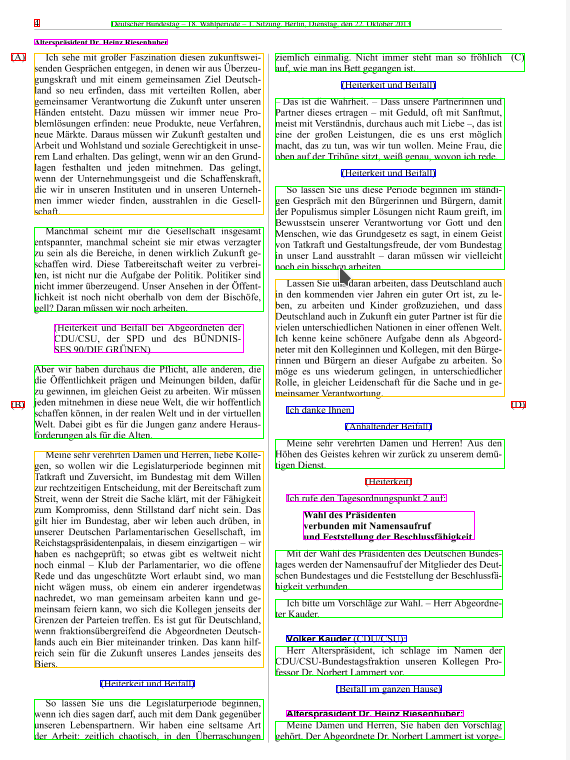
\includegraphics[height=0.5\textheight]{figures/cluster_example.png}
  \caption{An example of clustered blocks of text. Blocks with the same outline
    color belong to the same cluster.}
  \label{fig:clustered}
\end{figure}

\subsubsection{Hierarchical Agglomerative Clustering}
The first step is performed using hierarchical agglomerative clustering (HAC),
an unsupervised bottom-up clustering algorithm that constructs a hierarchical
tree of clusters (in this context referred to as a \emph{dendrogram}). An
example is shown in Figure~\ref{fig:hac}. The algorithm gets fed the individual
characters present in the PDF files, then iteratively groups the two closest
clusters (the initial inputs being regarded as clusters of one element) together
until only a single cluster remains. This process involves two parameters:
\begin{enumerate}
\item The distance function between two characters.
\item The distance function between two clusters of characters.
\end{enumerate}
The first parameter is trivially chosen to be the Euclidian distance between the
coordinates of the two characters. The second parameter is called the
\emph{linkage} and has several common options, the most basic of which are:
\begin{itemize}
\item Single-linkage: The distance between clusters is based on the closest two
  elements: \[ d(A, B) = \min \{ d(a, b) : a \in A, b \in B \} \]
\item Maximum-linkage: The distance between clusters is based on the furthest two
  elements: \[ d(A, B) = \max \{ d(a, b) : a \in A, b \in B \} \]
\item Average-linkage: The distance between clusters is based on the average
  distance of its elements:
  \[ d(A, B) = \frac{1}{|A||B|} \sum_{a \in A}\sum_{b \in B} d(a, b) \]
\end{itemize}
As per \textcite{klampfl2014unsupervised}, single-linkage clustering performs
best for this task due to its tendency to form long thin clusters. This is
beneficial since text is somewhat long and thin in nature (especially words and
sentences). As an additional bonus, while the general time complexity for HAC is
in $\mathcal{O}(n^3)$, single-linkage clustering can be done in
$\mathcal{O}(n^2)$ \citep{sibson1973slink}, making it far more usable on
realistic datasets.

\begin{figure}[htb]
  \centering
  \begin{subfigure}[b]{0.40\textwidth} 
    \centering
    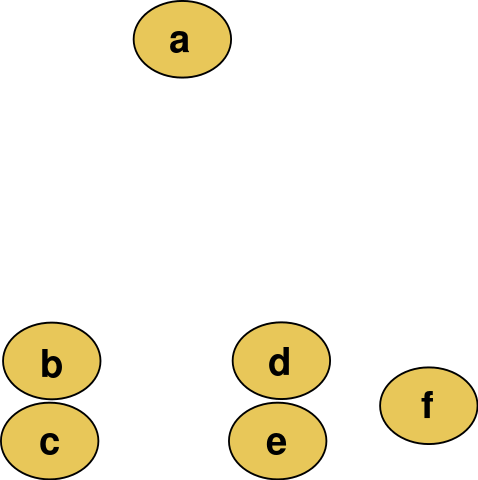
\includegraphics[width=\textwidth]{figures/dendrogram1.png}
    \caption{Before}
  \end{subfigure}
  \hspace{0.10\textwidth}
  \begin{subfigure}[b]{0.40\textwidth}
	\centering
    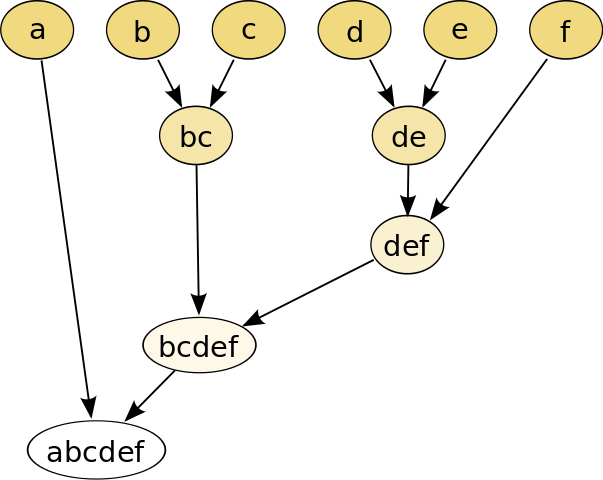
\includegraphics[width=\textwidth]{figures/dendrogram2.png}
    \caption{After}
  \end{subfigure}
  \caption{An example of hierarical agglomerative clustering, where the nodes
  are clustered by distance.}
  \label{fig:hac}
\end{figure}

After the dendrogram is constructed, it has to be cut at some level to obtain
the desired blocks of text. Clustering can optionally be rerun using the newly
found clusters as basic elements. This way, the document can incrementally be
clustered from characters into words, words into lines, and finally lines into
paragraphs. Both the level at which to cut the tree and the number of times to
recluster are determined by trial and error based on the particular set of
documents.

\subsubsection{K-Means}
The extracted blocks from the previous step are then clustered according to
their similarity based on the following metrics:
\begin{itemize}
  \item Width of the cluster
  \item Height of the cluster
  \item The ID of the most common font occurring in the cluster
  \item The size of the most common font occurring in the cluster
\end{itemize}
This is done using K-means clustering, with the value of $k$ being varied for
experimental purposes.

\subsection{Supervised}
\label{sec:sup}
After the data is augmented by the previously described clustering algorithms,
it's fed into a convolutional neural network for classification. Since the
source PDFs have a dual column layout with rather short lines, a sliding window
is used to add valuable context, with the center element in the window supplying
both the label (i.e.\ does or does not start a speech) and the cluster type. The
text content of this window is then entered into a standard convolutional neural
network architecture similar to the one proposed by \textcite{kim2014conv}.
First an embedding layer is used to learn a high-dimensional representation of
the words (no pre-trained embeddings were used because of both the specialized
political domain of the data as well as a lack of pre-trained German models),
followed by a number of Convolutional filters with max pooling. The output of
the filters is then concatenated into a single feature vector, which is amended
with the cluster type as an additional feature before feeding it into a standard
fully-connected neural network. This network features one hidden layer with a
ReLU activation ($\mathrm{relu}(x) = \max(0, x)$) and a single output node with a sigmoid
activation. The layout of this system is detailed in Figure~\ref{fig:model_full}
along with its parameters and their baseline value.

The network is trained for 50 epochs (which was found to be more than enough to
guarantee convergence in every test case), using the Adam\citep{adam} update
rule and binary cross-entropy as the loss function.  The loss will exhibit some
up and down fluctuations after the global minimum has been reached; to account
for this, the best loss so far along with the corresponding model parameters is
kept track of throughout the learning process.  Once 50 epochs have been
completed, the output is the model instantiated with the parameters
corresponding to the lowest loss that was obtained.

\begin{figure}[htbp]
  \centering
  \begin{subfigure}[b]{0.45\textwidth}
    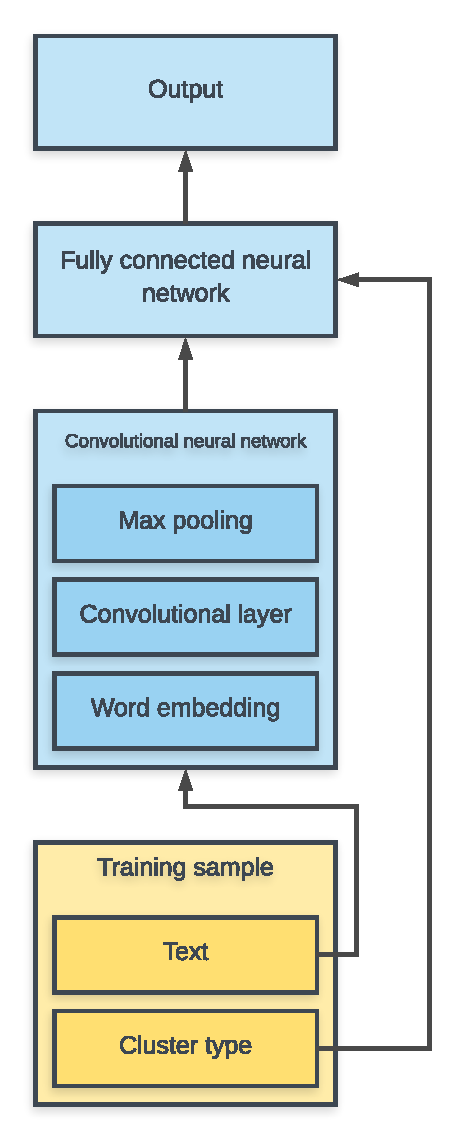
\includegraphics[width=\textwidth]{figures/nn_layout.pdf}
    \caption{The layout of the supervised portion of the system. The input data
      contains text and a cluster type assigned by the unsupervised portion. The
      text gets put into a convolutional neural network, the output of which is
      fed together with the cluster type into a fully connected neural network.
      The sigmoid function is applied to the output of this final neural network
    to obtain the classification.}
    \label{fig:nn_layout}
  \end{subfigure}
  \hspace{0.05\textwidth}
  \begin{subfigure}[b]{0.45\textwidth}
    \centering
    \begin{tabular}{lr}
      \toprule
      Parameter & Default value \\
      \midrule
      Window size & 3 \\
      Word embedding size & 300 \\
      Number of convolution filters & 100 \\
      Convolution filter sizes & 3, 5, 7 \\
      Convolution activation & ReLU \\
      Pooling type & 1-max \\
      Number of hidden layers & 1 \\
      Hidden layer size & 50 \\
      Number of outputs & 1 \\
      Output activation & Sigmoid \\
      \bottomrule
    \end{tabular}
    \caption{The default parameters used in the model.}
    \label{tbl:params}
  \end{subfigure}
  \caption{The model and its parameters.}
  \label{fig:model_full}
\end{figure}

\subsubsection{Convolutional Neural Networks}
\todo[inline]{This is kind of jumbled and out of place, might need to be deleted
or moved to an appendix or something.}
For the purposes of machine learning,
text produces 3-dimensional data: there is a feature vector for each word, and
some (either variable or predetermined through padding) amount of words per
text. This makes each training sample a 2-dimensional matrix, which then gets
stacked in the depth dimension to produce 3-dimensional training data. This is
troublesome as the standard machine learning algorithms work on 2-dimensional
data, assuming a feature vector for each sample rather than a matrix. There are
three common methods to deal with this:
\begin{itemize}
\item Bag of words
\item Convolutional neural networks
\item Recurrent neural networks
\end{itemize}

Aside from being completely different methods, they differ in a major way in how
they handle the sequential nature of text. The bag of words approach is the
simplest in that it simply disregards this sequential nature, instead creating
what is essentially a histogram of word occurrences. This downsamples each
sample from a feature matrix to a feature vector, allowing the use of normal
machine learning algorithms (commonly support vector machines). While the
sequential information can be kept to some degree by use histograms of $n$-grams
rather than words (unigrams), this causes the size of the input data to scale
exponentially with the value of $n$.

Convolutional neural networks (CNNs) work by taking a number of filters
(sometimes called kernels or feature maps) of a specified size and convolving
these over the input data. A simplified example using one filter is shown in
Figure~\ref{fig:cnn}.
\begin{figure}[htb]
  \centering
  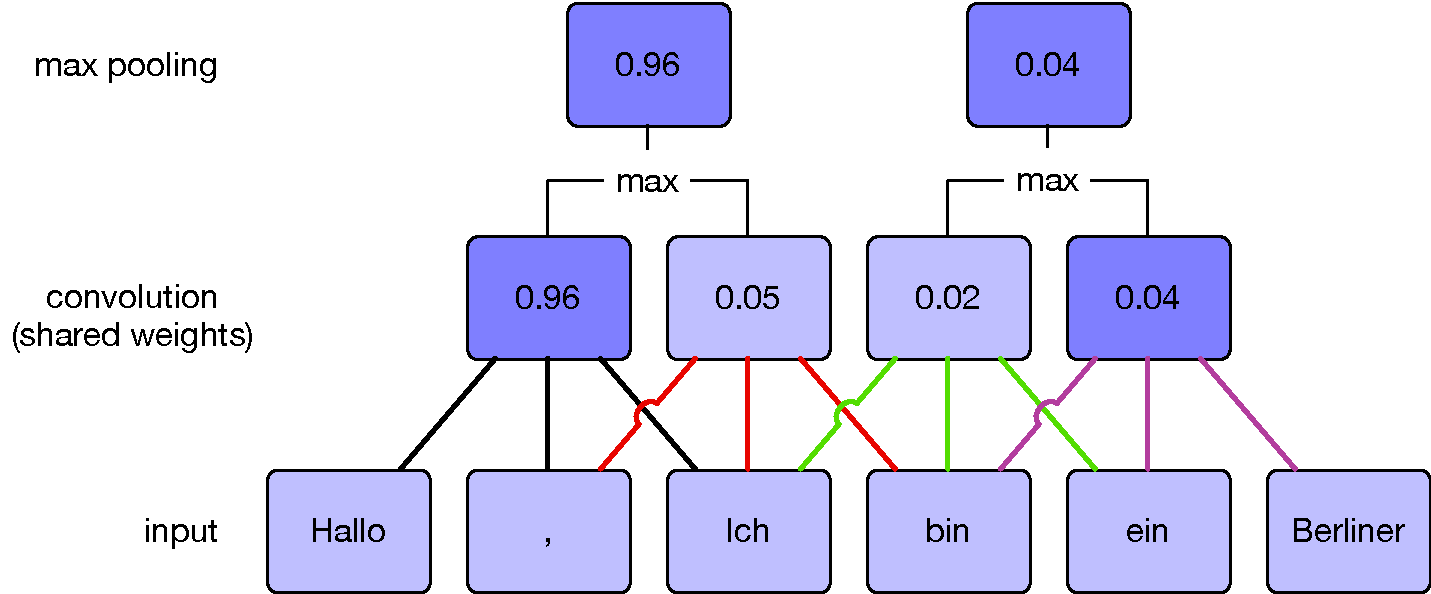
\includegraphics[width=\textwidth]{figures/cnn.pdf}
  \caption{A simplified convolutional neural network with one filter and
    max pooling.}
  \label{fig:cnn}
\end{figure}
In this example, the input text is convolved with a filter with a width of 3 and
a stride of 1 --- that is, each application of the filter considers three
subsequent input elements, after which the window is shifted one space to the
right. This filter is essentially a small neural network mapping three items to
one output value, whose weights are reused for each application of the filter.
Reusing the weights in this way (weight sharing) prevents the number of
parameters in the network from spiraling out of control.
\citep{lecun1995convolutional} After the application of this convolution layer,
the responses of the filter form a new sequence of roughly the same size as the
input (minus a few due to missing the edges). The next step is to downsample
this sequence by means of a \emph{max pooling} layer, which maps all values
within a window to the maximum value amongst those values. While conceptually
similar to a convolution, this step generally does not involve overlap, instead
either setting the stride to the same value as the window size (usually 2)
reducing the entire sequence to 1 value (1-max pooling). The reason for this is
twofold:
\begin{enumerate}
\item It downsamples the number of inputs, reducing the amount of parameters
  required further on in the network.
\item It adds translation invariance to the feature detected by this filter. The
  example filter of Figure~\ref{fig:cnn} appears to react strongly to the
  presence of the word ``Hallo''. Without the pooling layer, changing the
  location of the word ``Hallo'' in the input would similarly change the
  location of the high activation in the intermediate representation; this would
  be \emph{equivariance}. The more aggressively the pooling is applied, the
  higher the degree of invariance.
\end{enumerate}
This combination of convolution followed by pooling can be repeated multiple
times as desired or until there is only a single value left as output from the
filter. Finally, the outputs of all filters are concatenated and fed into a
standard feedforward neural network.

While CNN architectures in computer vision are generally very deep, they tend to
be very shallow in natural language processing; commonly just a single
convolution followed by 1-max pooling \citep{zhang2015conv}. Since this
particular task at first glance appears to be fairly reliant on word position
(e.g.\ a colon at the end of a sentence very often indicates the start of a
speech, a colon in the middle almost certainly does not), the degree of pooling
will be experimented with.

\subsubsection{Difference between convolutional and recurrent neural networks}
Recurrent neural networks (in particular LSTMs or GRUs) are seemingly the most
natural fit for language processing, since they process an entire sequence and
are therefore fully conditioned on the word order (as opposed to the
convolutional neural networks which tend to learn translation invariant ngram
features). Regardless, convolutional neural networks will be used in this
research. This choice is based on two factors:
\begin{enumerate}
\item In practise, the performance for classification tasks does not differ
  between the two types of networks.\citep{cnnrnn}
\item The computations in convolutional networks are highly independent of
  each other, allowing for great paralellization (in particular with regards to
  running on a GPU). In contrast, LSTMs are bottlenecked by the fact that each
  calculation is dependent on the previous calculations. As a result, CNNs
  achieve far higher training speeds.\citep{facebook}
\end{enumerate}

%%% Local Variables:
%%% mode: latex
%%% TeX-master: "report"
%%% End:
